\chapter{Estudo do ambiente da empresa}
\label{cap:estudodecaso}

Este capítulo apresentará a estrutura da empresa que será objetivo de estudo neste trabalho. Esta é uma empresa que fornece serviços de 
hospedagens e também está associada a um provedor de Internet\footnote[1]{É importante salientar que esse provedor utiliza a maior parte dos 
serviços da empresa, pois possui maior número de clientes.}. A empresa possui grande parte de seus clientes localizados na serra do 
Rio Grande do Sul, sendo que atualmente essa empresa possui aproximadamente 9000 clientes. A sede da empresa está localizada na cidade de 
Garibaldi, além disso possui quatro filiais no estado, atendendo aproximadamente xx?? cidades.

A empresa oferece serviços pela internet aos seus clientes, sendo eles: hospedagens de sites, banco de dados, \textit{e-mail}, sistemas de gestão, 
\textit{e-mail marketing}, \textit{backup}, \textit{máquinas virtuais}, autenticação via \ac{ADSL}, rádio \textit{online} e telefonia.
Além disso, o provedor associado fornece aos seus clientes acesso à internet via rádio e acesso à internet por meio de fibra óptica.
A maioria dos serviços são fornecidos por meio de \textit{softwares} de código aberto.

Atualmente a empresa possui redundância de refrigeração e de energia, como pode ser observado na Figura \ref{fig:insteletrica}. 
A redundância de refrigeração é composta por dois ares-condicionados (destacados com a cor azul). 

\begin{figure}[h!]
 \centering
 \fcolorbox{black}{white}{
  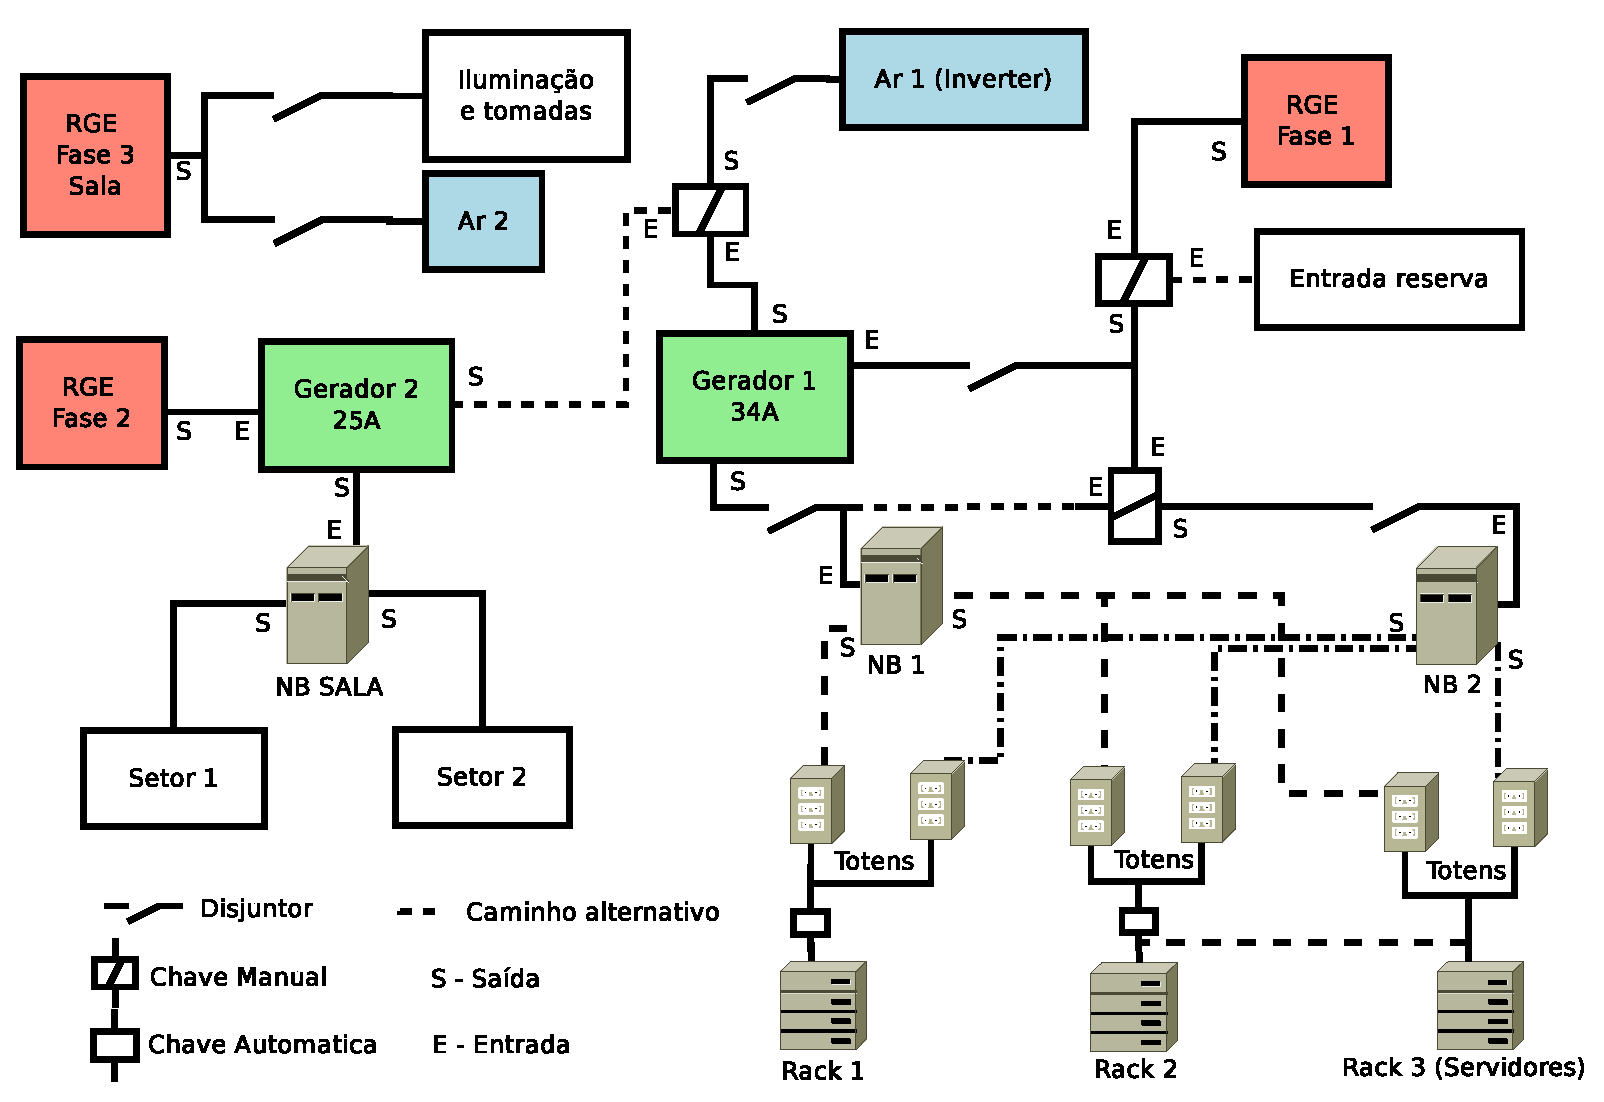
\includegraphics[width=320px]{img/insteletrica.eps}
 }
 \caption{Diagrama de instalação elétrica.}
 \label{fig:insteletrica}
\end{figure}

A redundância de energia é feita através de três \textit{nobreaks}, sendo que dois deles (identificados como NB 1 e NB 2) são utilizados para 
alimentação dos servidores e outros equipamentos como por exemplo roteadores, de forma que caso um falhe o outro alimente todos os equipamentos. 
O terceiro \textit{nobreak} (identificado como NB Sala) é utilizado para alimentar os computadores dos funcionários de dois setores da empresa. 
Ligado aos \textit{nobreaks} estão seis \textit{totens}\footnote[1]{Totens são torres que possuem tomadas para plugar os equipamentos},
nesses \textit{totens} são ligados os equipamentos e servidores que estão montados nos \textit{racks}. 
Além disso, existem a entrada de energia, com três fases (destacadas na cor vermelho), e dois geradores (destacados na cor verde) que suprem a 
necessidade de consumo de energia elétrica do ambiente.

Nas próximas seções será feita uma descrição da estrutura da empresa. Na Seção \ref{section:fisico} será descrito a instalação física dos 
servidores, com suas estruturas e suas configurações. Na Seção \ref{section:servsemvirt} será descrito os servidores que não utilizam virtualização,
ou seja, possuem os seus serviços instalados diretamente sobre o sistema operacional.
Na Seção \ref{section:servvirt} será descrito a estrutura de virtualização e todos os serviços fornecidos pelos servidores. 
E na Seção \ref{section:servcrit} será feito a seleção dos serviços críticos através de alguns critérios.

\section{Instalação física}
\label{section:fisico}

A estrutura atual da empresa é composta por quatorze servidores físicos. 
A configuração de \textit{hardware} desses servidores pode ser encontrada na Tabela \ref{tab:servfisicos}, onde tem-se o nome do servidor, 
o modelo, a configuração dos processadores, quantidade de memória, número de discos e a capacidade unitária de cada disco.

\begin{table}[h!]
\caption{Configuração dos servidores físicos.}
\label{tab:servfisicos}
\begin{center}
\def\arraystretch{1}
\setlength{\tabcolsep}{0.15cm}
\begin{tabular}{|l|l|p{5.1cm}|l|p{2.1cm}|}\hline
Servidor & Modelo & Processador & Memória & Disco\\\hline
Bello & & 1 x Intel Core 2 Duo E6750 2.66 GHz & 2 GB DDR2 & 5,5 TB SATA\\\hline
Cacti & Dell PowerEdge 2950 & 2 x Intel Xeon E5310 1.60 GHz & 12 GB DDR2 & 2 x 73 GB SAS\\\hline
Dati & Dell PowerEdge 1850 & 2 x Intel Xeon 3.20 GHz & 4 GB DDR2 & 2 x 146 GB SCSI\\\hline
Monit & & 1 x Intel Core 2 Quad Q9550 2.83 GHz & 4 GB DDR2 & 120 GB SSD\\\hline
Nino & & 1 x Intel Core 2 Duo E4500 2.20 GHz & 4 GB DDR2 & 500 GB SATA\\\hline
Sfrunhon & & 1 x Intel Xeon X3330 2.66 GHz & 8 GB DDR2 & 750 GB SATA\\\hline
Vigilante & & 1 x Intel Pentium Dual E2180 2.00 GHz & 4 GB DDR2 & 2,5 TB SATA\\\hline
Brina & Dell PowerEdge 2950 & 2 x Intel Xeon E5410 2.33 GHz & 24 GB DDR2 & 6 x 300 GB SAS\\\hline
Fulmine & IBM System x3650 M4 & 1 x Intel Xeon E5-2650 2.00 GHz & 32 GB DDR3 & 6 x 2 TB SATA\\\hline
Piova & Dell PowerEdge R410 & 2 x Intel Xeon E5530 2.40 GHz & 32 GB DDR3 & 4 x 500G SATA\\\hline
Raggio & HP ProLiant DL360 G7 & 2 x  Intel Xeon E5630 2.53 GHz & 32 GB DDR3 & 4 x 300 GB SAS\\\hline
Tempesta & Dell PowerEdge R620 & 2 x Intel Xeon E5-2620 2.00 GHz & 32 GB DDR3 & 5 x 1 TB SATA 3 x 1,2 TB SAS\\\hline
Tuono & HP ProLiant DL380 G7 & 2 x Intel Xeon E5649 2.53 GHz & 32 GB DDR3 & 6 x 300 GB SAS 2 x 146 GB SAS\\\hline
Venti & Dell PowerEdge R210 II & 1 x Intel Xeon E3-1220 3.10 GHz & 16 GB DDR3 & 2 x 3 TB SATA\\\hline
\end{tabular}
\end{center}
\end{table}

Todos os servidores estão ligados ao \textit{switch}, que provê aos servidores acesso à internet através de um roteador. Para os servidores 
mais importantes são utilizados dois cabos de rede que estão ligados a um \textit{switch} \textit{gigabit}, assim possibilitando
a configuração de \textit{link aggregation}, ou seja, permite configurar mais de uma interface de rede física em uma interface agregada, com isso 
pode-se dobrar a capacidade de tráfego de dados e obter redundância de interfaces. 
O diagrama da Figura \ref{fig:servfisicos} demonstra uma visão geral da estrutura física dos servidores da empresa. 

\begin{figure}[h!]
 \centering
 \fcolorbox{black}{white}{
  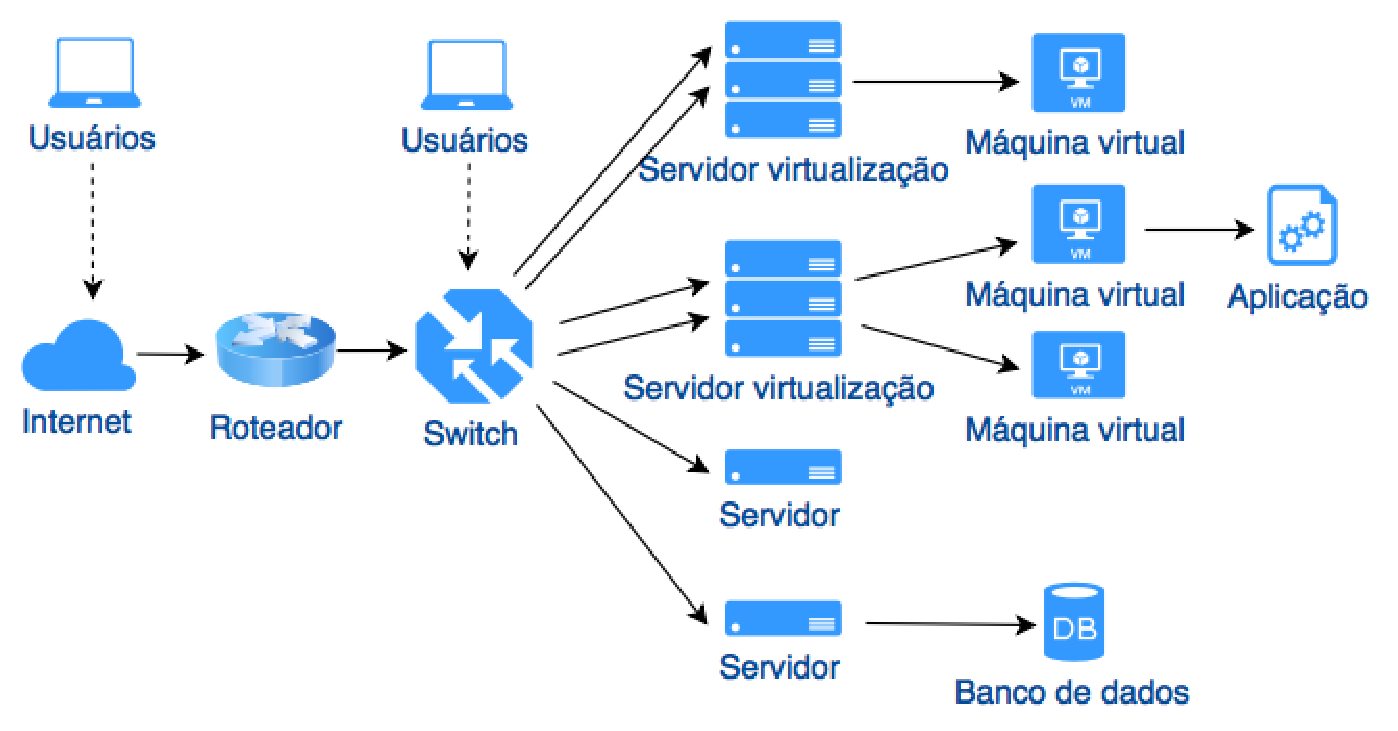
\includegraphics[width=380px]{img/servfisicos.eps}
 }
 \caption{Modelo de estrutura física.}
 \label{fig:servfisicos}
\end{figure}

A Figura \ref{fig:servrack} demonstra, através de uma foto, todos os servidores, inclusive o \textit{switch}, montados em um \textit{rack}.

\begin{figure}[h!]
 \centering
 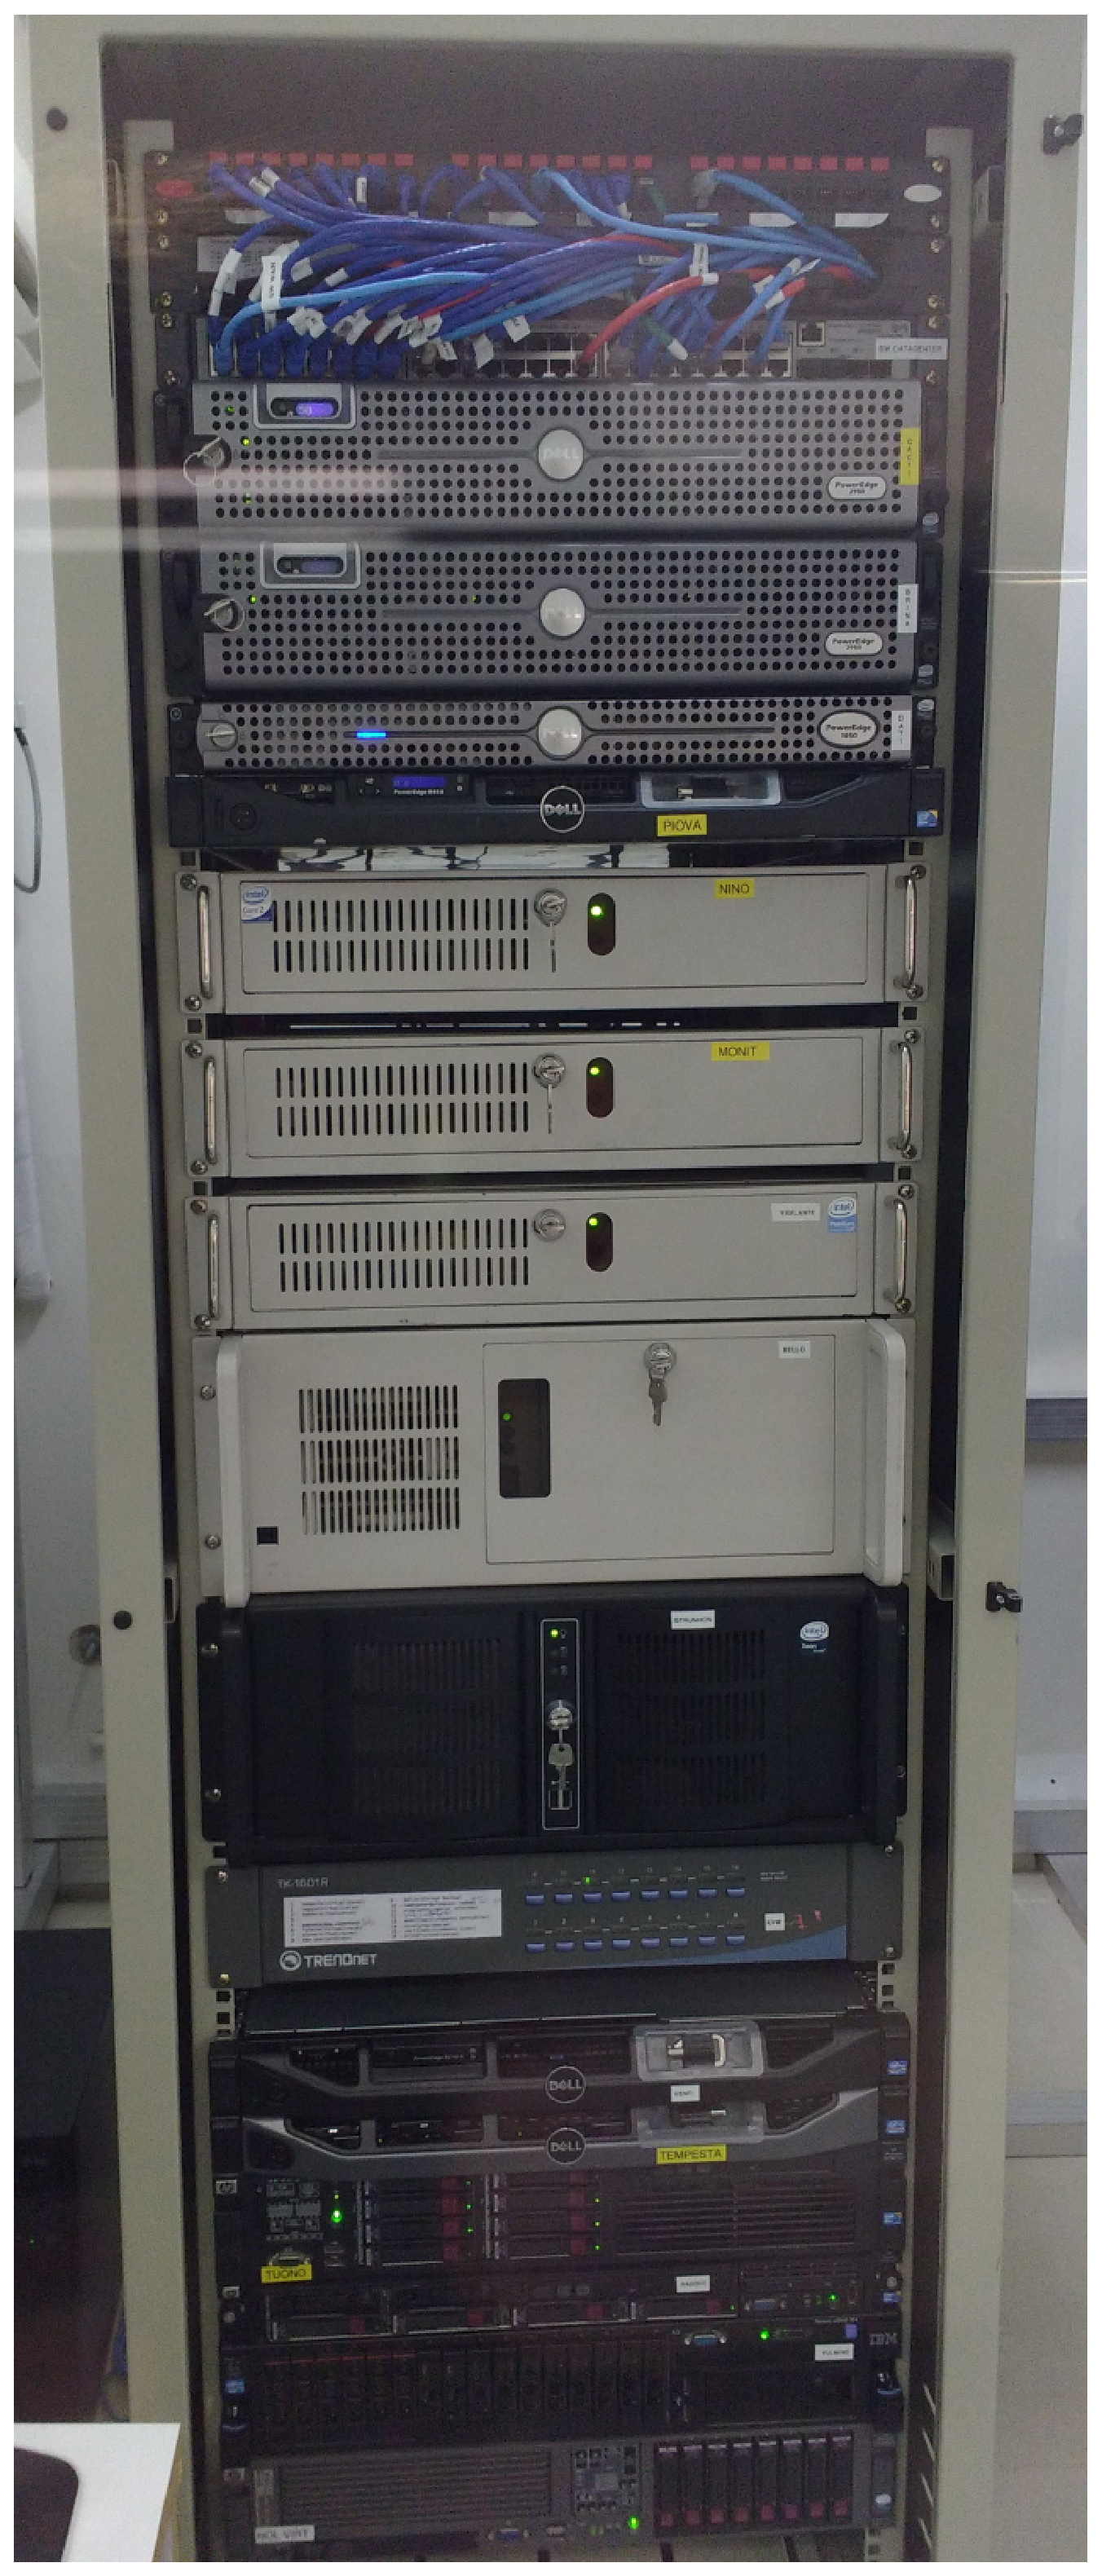
\includegraphics[width=120px]{img/servrack.eps}
 \caption{Imagem do \textit{rack} e dos servidores.}
 \label{fig:servrack}
\end{figure}

\section{Servidores sem virtualização}
\label{section:servsemvirt}

Atualmente existem sete servidores que possuem serviços onde executam sobre o sistema operacional nativo, ou seja, sem virtualização. 
Eles são os sete primeiros servidores da Tabela \ref{tab:servfisicos}, e são listados a seguir:
\begin{itemize}
 \item Bello: esse servidor possui o sistema operacional \textit{Ubuntu 14.04 \ac{LTS}} \cite{ubuntu}. Sua função é armazenar dados de 
 \textit{backup}, para isso ele possui a ferramenta \textit{Bacula Storage 5.2.6} \cite{bacula} instalado, que o possibilita fazer esse 
 armazenamento. Sendo que a ferramenta que é responsável por fazer o \textit{backup} está instalada em um outro servidor que será detalhado na 
 Seção \ref{section:serv_venti};
 
 \item Cacti: um dos servidores de monitoramento da rede do provedor. Esse utiliza a distribuição \textit{CentOS 6.6} \cite{centos} e executa a 
 aplicação \textit{Cacti 0.8.8b} \cite{cacti}, que é uma ferramenta de código aberto desenvolvida para monitorar qualquer equipamento de rede que 
 suporte o protocolo \ac{SNMP}. Ela monitora atualmente a maior parte da rede \textit{core} e a rede \textit{backbone} tanto dos clientes de 
 internet via rádio, como de fibra óptica;
 
 \item Dati: é o servidor de banco de dados principal. Esse possui o sistema operacional \textit{Ubuntu 14.04 \ac{LTS}} \cite{ubuntu}. 
 O serviço que executa sobre esse servidor é um sistema gerenciador de banco de dados \textit{MySQL 5.5.49} \cite{mysql}, que armazena os dados 
 das aplicações de \textit{ZoneMinder} \cite{zoneminder} (servidor de câmeras) e \textit{Icewarp Server} (servidor de \textit{e-mail}), que serão 
 detalhados na Seção \ref{section:servvirt};
 
 \item Monit: esse servidor faz o monitoramento dos demais servidores. Ele possui o sistema operacional \textit{Ubuntu 12.04 \ac{LTS}} 
 \cite{ubuntu}, executando as aplicações \textit{Nagios 3.2.3} \cite{nagios} e \textit{Munin 1.4.6} \cite{munin}, ambos \textit{softwares} livres. 
 O \textit{Nagios} monitora o \textit{hardware} e os serviços que estão executando em cada servidor. Para alguns serviços é utilizado um cliente 
 \textit{Nagios}. O segundo, \textit{Munin}, é responsável por gerar gráficos de monitoramento. Com ele pode-se criar, por exemplo, gráficos 
 com a utilização: do processador, memória, disco, temperatura e velocidade dos \textit{fans};
 
 \item Nino: esse é o servidor utilizado pelo setor de desenvolvimento de \textit{software}. Suas aplicações executam sobre o sistema operacional 
 \textit{Ubuntu 14.04 \ac{LTS}} \cite{ubuntu}, sendo que os serviços fornecidos pelo servidor são um servidor \textit{web} (\textit{Apache 2.4.7} 
 \cite{apache} e \textit{\ac{PHP} 5.5.9} \cite{php}), sistema gerenciador de banco de dados (\textit{MySQL 5.5.49} \cite{mysql} e 
 \textit{PostgreSQL 9.3.13} \cite{postgres}), compartilhamento de arquivos (\textit{Samba 4.3.9} \cite{samba}), controle de versões de 
 \textit{software} (\textit{\ac{SVN} 1.8.8} \cite{svn}), gerenciador de \textit{bugs} (\textit{Trac 1.0.1} \cite{trac}) e mensagens instantâneas 
 (\textit{Ejabberd 2.1.11} \cite{ejabberd});
 
 \item Sfrunhon: outro servidor de monitoramento da rede do provedor. Esse utiliza a distribuição \textit{CentOS 6.3} \cite{centos} e executa a 
 aplicação \textit{Cacti 0.8.8a} \cite{cacti}. Esse servidor monitora atualmente o tráfego dos clientes, tanto de internet via rádio, como de 
 fibra óptica;
 
 \item Vigilante: esse servidor é responsável por capturar e armazenar \textit{streaming} de vídeo das câmeras do provedor. Ele possui o sistema 
 operacional \textit{Ubuntu 14.04 \ac{LTS}} \cite{ubuntu} e executa a aplicação \textit{ZoneMinder 1.29} \cite{zoneminder}, que é o 
 \textit{software} responsável pela captura e armazenamento das as imagens das câmeras do provedor.
\end{itemize}

\section{Servidores com virtualização}
\label{section:servvirt}

Os servidores de virtualização possuem suas respectivas \ac{VM}s, que executam aplicações. Para virtualização utiliza-se o hipervisor 
\ac{KVM} e a ferramenta \textit{QEmu}, sendo que ambos são projetos de \textit{software} livre. Procurou-se manter um ambiente homogêneo 
com o objetivo de facilitar a manutenção, para isso utilizou-se o mesmo hipervisor e o mesmo sistema operacional para os servidores de virtualização
(hospedeiros). 
Esse sistema operacional é o sistema de código aberto \textit{Ubuntu 14.04 \ac{LTS}} \cite{ubuntu}.
Além disso, esses servidores possuem redundância de \textit{hardware}, com fonte de alimentação e discos configurados através de um \ac{RAID}. 
Em servidores com mais de dois discos geralmente é utilizado \ac{RAID} 5. Já em servidores que possuem apenas dois discos é utilizado \ac{RAID} 1 
(espelhamento de discos). O ambiente também possui uma redundância do cabeamento, como visto anteriormente.

A empresa fornece serviços diversos, desde hospedagens de sites até \ac{DNS} recursivo para o provedor de internet. Atualmente sete servidores 
são utilizados para virtualizar sistemas, que são os últimos sete servidores da Tabela \ref{tab:servfisicos}, sendo que existem quarenta e seis 
\ac{VM}s distribuídas entre os sete servidores de virtualização. Nas próximas seções serão descritos esses servidores, suas respectivas 
máquinas virtuais e serviços.

\subsection{Servidor Brina}
\label{section:serv_brina}

O servidor Brina possui duas \ac{VM}s, como pode ser visto na Figura \ref{fig:servidor_brina} juntamente com seus respectivos serviços. 
Esses serviços são listados a seguir:

\begin{figure}[h!]
 \centering
 \fcolorbox{black}{white}{
  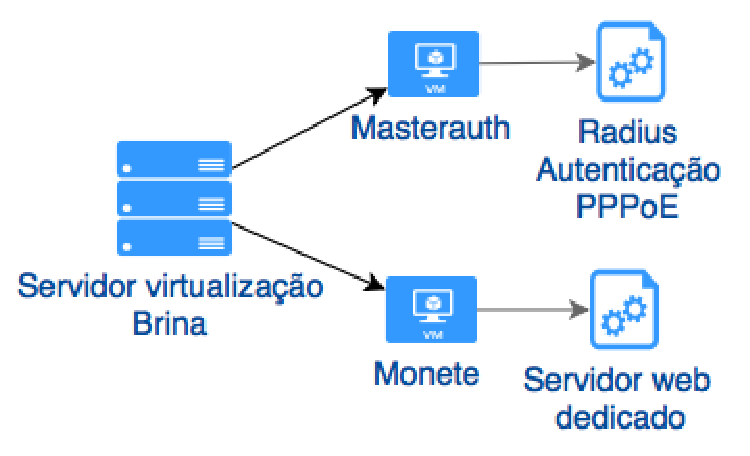
\includegraphics[width=180px]{img/servidor_brina.eps}
 }
 \caption{Servidor de virtualização Brina.}
 \label{fig:servidor_brina}
\end{figure}

\begin{itemize}
 \item \textit{Masterauth}: sua configuração é 1 \textit{core} para processamento, 1,5 GB de memória e 8 GB de disco. O sistema operacional é o 
 \textit{Ubuntu 14.04 \ac{LTS}} \cite{ubuntu}, sendo que esse servidor fornece o serviço de autenticação \ac{PPPoE} para apenas uma parte dos 
 clientes do provedor utilizando \textit{Radius} (\textit{Freeradius 2.1.12} \cite{freeradius});
 
 \item \textit{Monete}: sua configuração é 1 \textit{core} de processamento, 3 GB de memória e 50 GB de disco. Esse servidor possui o 
 sistema operacional \textit{Ubuntu 14.04 \ac{LTS}} \cite{ubuntu}, sendo um servidor \textit{web} dedicado para o site do provedor, com 
 configurações personalizadas. Para isso ele utiliza os \textit{softwares} \textit{Apache 2.4.7} \cite{apache}, \textit{\ac{PHP} 5.5.9} \cite{php} 
 (com \textit{PHP-FPM 5.59}) e \textit{MySQL 5.5.49} \cite{mysql}.
\end{itemize}

\subsection{Servidor Fulmine}
\label{section:serv_fulmine}

O servidor Fulmine possui dez \ac{VM}s, como pode ser visto na Figura \ref{fig:servidor_fulmine} juntamente com seus respectivos serviços. 
Esses serviços são listados a seguir:

\begin{figure}[h!]
 \centering
 \fcolorbox{black}{white}{
  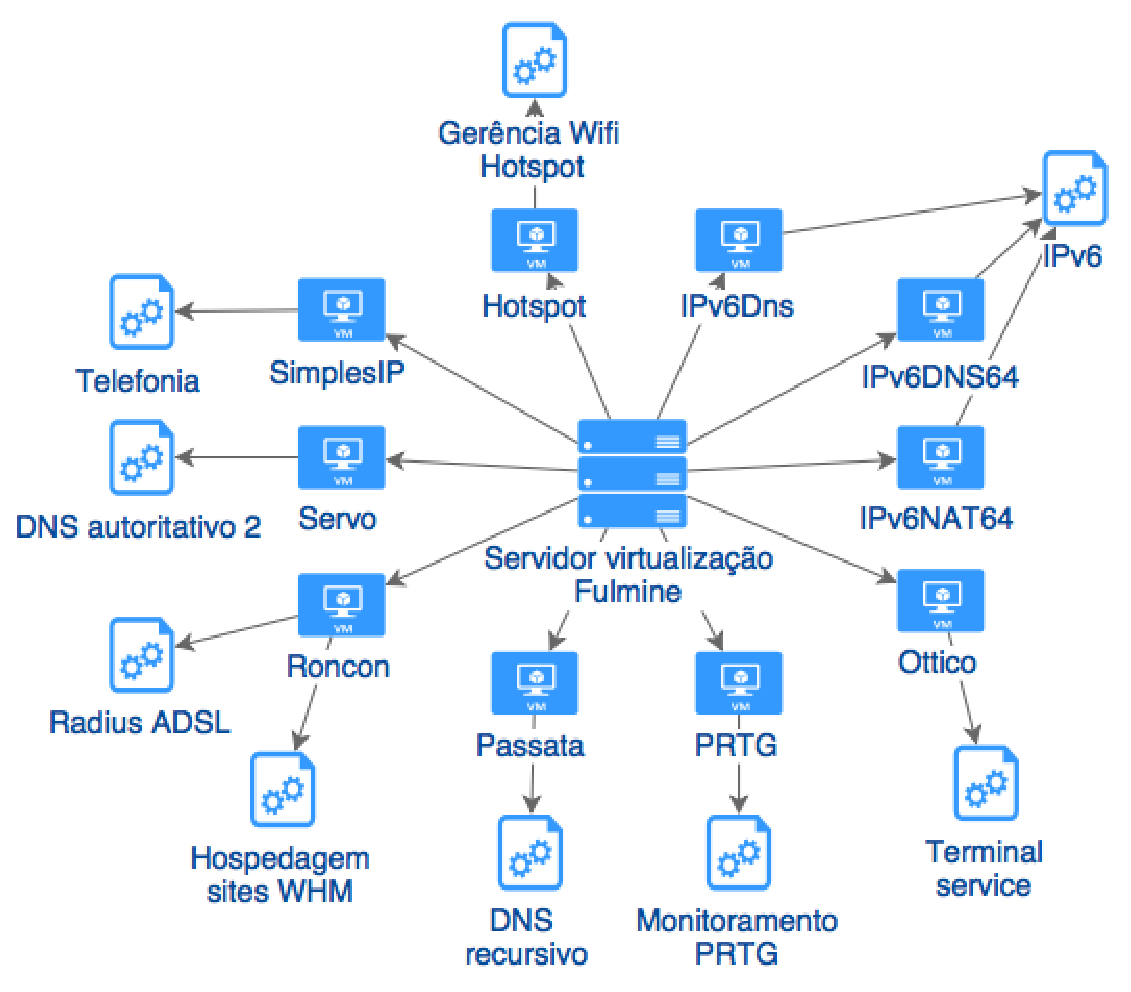
\includegraphics[width=310px]{img/servidor_fulmine.eps}
 }
 \caption{Servidor de virtualização Fulmine.}
 \label{fig:servidor_fulmine}
\end{figure}

\begin{itemize}
 \item \textit{Hotspot}: sua configuração é 1 \textit{core} para processamento, 1,5 GB de memória e 8 GB de disco. Esse servidor possui o 
 sistema operacional \textit{Ubuntu 14.04 \ac{LTS}} \cite{ubuntu}, sendo que esse é o servidor de gerência de equipamentos da \textit{Ubiquiti} 
 que fazem \textit{hotspot}, que é uma maneira de disponibilizar a tecnologia \textit{Wi-fi} para prover acesso à internet em ambientes públicos, 
 sendo utilizado pelo provedor;
 
 \item \textit{IPv6Dns}, \textit{IPv6Dns64} e \textit{IPv6Nat64}: suas configurações são 1 \textit{core} para processamento, 1 GB de memória e 
 8 GB de disco. O sistema operacional é o \textit{Ubuntu 14.04 \ac{LTS}} \cite{ubuntu}, sendo que esses servidores fornecem o serviço de \ac{DNS} 
 e \ac{NAT} para navegação \ac{IPv6} do provedor;
 
 \item \textit{Ottico}: esse servidor possui 2 \textit{cores} para processamento, 4 GB de memória e 50 GB de disco. O servidor possui o sistema 
 operacional \textit{Windows 2007 Server Standard} e possui o serviço de \textit{terminal service} para suporte e gerência de fibra óptica do 
 provedor;
 
 \item \ac{PRTG}: esse servidor possui 2 \textit{cores} para processamento, 4 GB de memória e 100 GB de disco. O servidor possui o sistema 
 operacional \textit{Windows 2008 Server R2} e sua função é fazer o monitoramento de tráfego e equipamentos da rede \textit{core} do provedor;
 
 \item \textit{Passata}: esse servidor possui 2 \textit{cores} para processamento, 3 GB de memória e 20 GB de disco. O servidor possui o 
 sistema operacional \textit{Ubuntu 14.04 \ac{LTS}} \cite{ubuntu} e fornece o serviço de \ac{DNS} recursivo, através do \textit{software} 
 \textit{Bind 9.9.5} \cite{bind}. Esse é o servidor primário de \ac{DNS}, sendo o mais importante para navegação dos clientes de todo o provedor;
 
 \item \textit{Roncon}: esse servidor possui 4 \textit{cores} para processamento, 6 GB de memória e 400 GB de disco. Ele possui o sistema
 operacional \textit{Red Hat 5.11} \cite{redhat} e provê acesso a sites \textit{web} desenvolvidos com a linguagem \ac{PHP}. Nele está instalado 
 o \textit{software} \ac{WHM} \cite{whm}, que faz a gerência dos serviços de hospedagens de sites e banco de dados. Além disso, encontra-se 
 disponível a ferramenta \textit{cPanel}, que faz parte do \ac{WHM} e que fornece a gerência de cada hospedagem de site para seu respectivo 
 desenvolvedor. Para fornecer essa hospedagem os seguintes \textit{softwares} estão instalados e configurados: \textit{Apache 2.2.26} \cite{apache}, 
 \textit{\ac{PHP} 5.3.27} \cite{php}, \textit{MySQL 5.1.73} \cite{mysql} e \textit{PostgreSQL 8.4.20} \cite{postgres}.
 Além da hospedagem, esse servidor fornece o serviço de autenticação \ac{ADSL} de terceiros utilizando o \textit{software} \textit{Radius} 
 (\textit{Freeradius 1.1.3} \cite{freeradius});
 
 \item \textit{Servo}: sua configuração é 1 \textit{core} para processamento, 2 GB de memória e 30 GB de disco. Esse servidor possui o 
 sistema operacional \textit{CentOS 6.8} \cite{centos}, sendo que esse servidor fornece, através do \textit{software} \textit{Bind 9.8.2} 
 \cite{bind}, o serviço de \ac{DNS} autoritativo e é o servidor \ac{DNS} secundário dos domínios hospedados pela empresa;
 
 \item \textit{SimplesIP}: esse servidor possui 2 \textit{cores} para processamento, 3 GB de memória e 80 GB de disco. O servidor possui 
 o sistema operacional \textit{CentOS 6.6} \cite{centos} e é o servidor de telefonia do provedor. Esse utiliza como base o \textit{software} 
 livre \textit{Asterisk 1.8.32} \cite{asterisk}.
\end{itemize}

\subsection{Servidor Piova}
\label{section:serv_piova}

O servidor Piova possui nove \ac{VM}s, como pode ser visto na Figura \ref{fig:servidor_piova} juntamente com seus respectivos serviços. 
Esses serviços são listados a seguir:

\begin{figure}[h!]
 \centering
 \fcolorbox{black}{white}{
  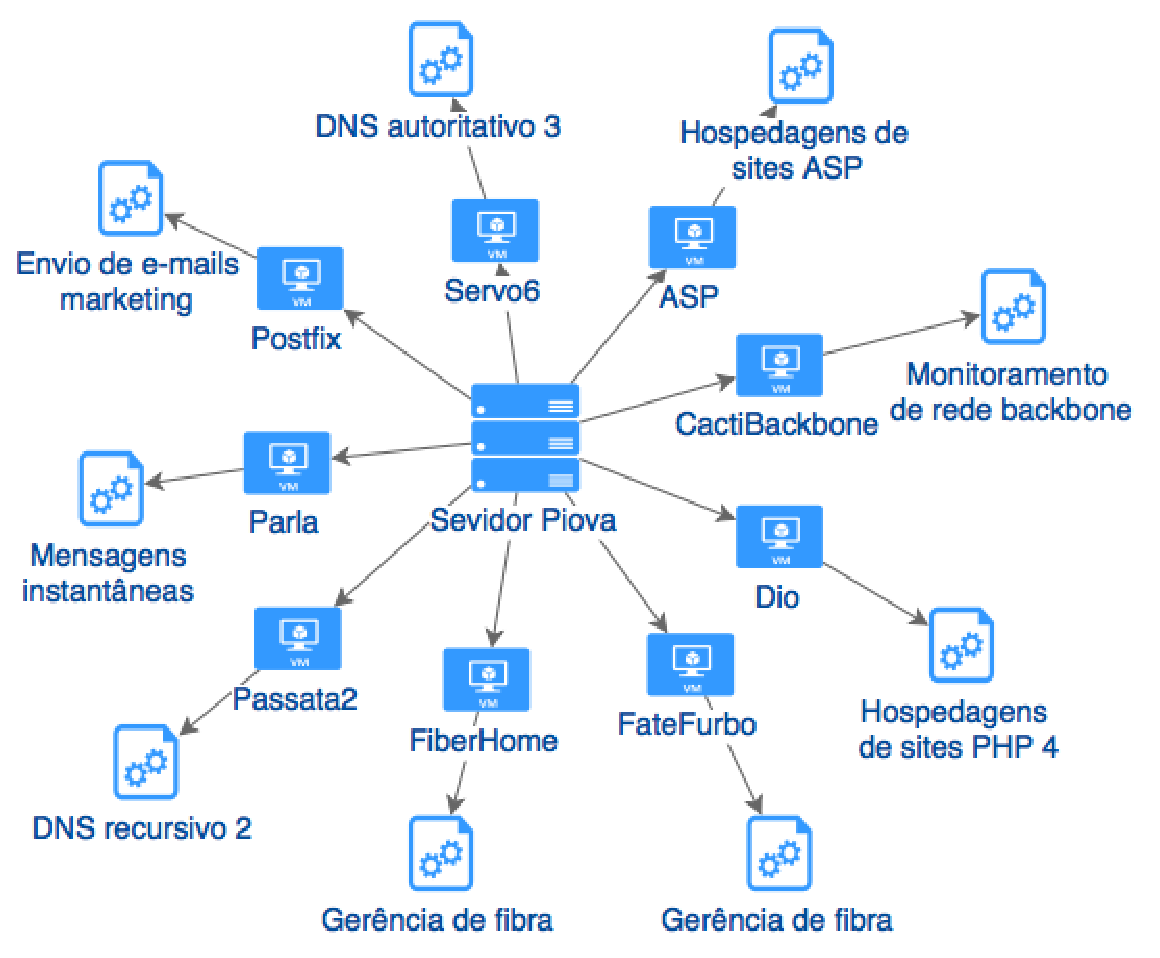
\includegraphics[width=320px]{img/servidor_piova.eps}
 }
 \caption{Servidor de virtualização Piova.}
 \label{fig:servidor_piova}
\end{figure}

\begin{itemize}
 \item \textit{ASP}: esse servidor possui 1 \textit{core} para processamento, 1 GB de memória e 50 GB de disco. O servidor possui o sistema 
 operacional \textit{Windows 2008 Server R2} e provê acesso a sites \textit{web} desenvolvidos com a linguagem \ac{ASP} \cite{asp}, através do
 \textit{software} \textit{\ac{IIS} 7.5} \cite{iis}. Esse servidor hospeda um número bem baixo de sites;
 
 \item \textit{CactiBackbone}: esse servidor possui 1 \textit{core} para processamento, 1 GB de memória e 20 GB de disco. Ele é um servidor
 de monitoramento da rede do provedor. Esse utiliza a distribuição \textit{CentOS 6.3} \cite{centos} e executa a aplicação \textit{Cacti 0.8.8a}
 \cite{cacti}. Essa aplicação monitora atualmente uma parte da rede \textit{backbone} do provedor;
 
 \item \textit{Dio}: esse servidor possui 1 \textit{core} para processamento, 1 GB de memória e 17,8 GB de disco. O servidor possui o sistema 
 operacional \textit{Ubuntu 6.06 \ac{LTS}} \cite{ubuntu} e fornece serviço de hospedagens de sites desenvolvidos com a linguagem \ac{PHP} 
 versão 4.4.2. Esses sites são mantidos em um servidor separado devido a incompatibilidade com a versão 5. Esse servidor armazena 
 aproximadamente 10 sites;
 
 \item \textit{FateFurbo}: sua configuração é 2 \textit{cores} para processamento, 4 GB de memória e 80 GB de disco. O sistema operacional é o 
 \textit{Ubuntu 14.04 \ac{LTS}} \cite{ubuntu} e possui um \textit{software} proprietário da empresa \textit{Padtec}, e que faz a gerência de uma 
 parte pequena da fibra óptica do provedor;
 
 \item \textit{FiberHome}: sua configuração é 2 \textit{cores} para processamento, 2 GB de memória e 60 GB de disco. Esse servidor possui o sistema 
 operacional \textit{Windows XP} e possui o \textit{software} \textit{ANM 2000} instalado, para fazer a gerência da fibra óptica do provedor;
 
 \item \textit{Parla}: sua configuração é 1 \textit{core} de processamento, 1 GB de memória e 8 GB de disco. Ele possui o sistema
 operacional \textit{Ubuntu 14.04 \ac{LTS}} \cite{ubuntu} e provê um serviço de mensagens instantâneas, baseado no protocolo \ac{XMPP}. Esse 
 serviço é utilizado para comunicação entre funcionários da empresa e do provedor. O \textit{software} utilizado é o \textit{Ejabberd 2.1.11}
 \cite{ejabberd}, que também é um \textit{software} livre;

 \item \textit{Passata2}: esse servidor possui 1 \textit{core} para processamento, 2 GB de memória e 20 GB de disco. Esse servidor possui o 
 sistema operacional \textit{Ubuntu 14.04 \ac{LTS}} \cite{ubuntu} e fornece o serviço de \ac{DNS} recursivo, através do \textit{software} 
 \textit{Bind 9.9.5} \cite{bind}. Esse é o servidor secundário de \ac{DNS} do provedor;
 
 \item \textit{Postfix}: sua configuração é 1 \textit{core} para processamento, 768 MB de memória e 50 GB de disco. Esse servidor possui o 
 sistema operacional \textit{Ubuntu 14.04 \ac{LTS}} \cite{ubuntu} e é responsável pelo envio de \textit{e-mails}, através do \textit{software} 
 \textit{Postfix 2.11} \cite{postfix}. Os \textit{e-mails} enviados por esse servidor são gerados por uma ferramenta de \textit{e-mail marketing}, que foi
 desenvolvida pela empresa. Esse servidor faz o envio de \textit{e-mails} em massa para divulgação de informações ou produtos;
 
 \item \textit{Servo6}: sua configuração é 1 \textit{core} para processamento, 1,5 GB de memória e 30 GB de disco. Esse servidor possui o 
 sistema operacional \textit{CentOS 6.8} e fornece, através do \textit{software} \textit{Bind 9.8.2} \cite{bind}, o serviço de \ac{DNS} 
 autoritativo, sendo o servidor de \ac{DNS} terciário dos domínios hospedados pela empresa.
\end{itemize}

\subsection{Servidor Raggio}
\label{section:serv_raggio}

O servidor chamado Raggio executa doze \ac{VM}s (Figura \ref{fig:servidor_raggio}), que fornecem os serviços de virtualização para algumas empresas,
sendo que as máquinas virtuais são instaladas com o sistema operacional da preferência do cliente, e são disponibilizadas através de um serviço 
de acesso remoto, como por exemplo, através de \ac{SSH}.

\begin{figure}[h!]
 \centering
 \fcolorbox{black}{white}{
  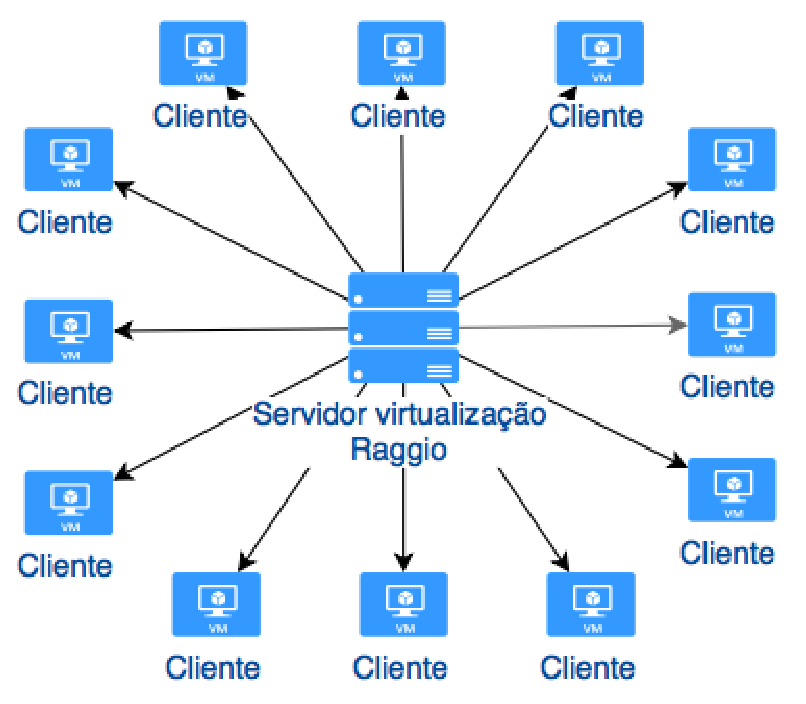
\includegraphics[width=220px]{img/servidor_raggio.eps}
 }
 \caption{Servidor de virtualização Raggio.}
 \label{fig:servidor_raggio}
\end{figure}

\subsection{Servidor Tempesta}
\label{section:serv_tempesta}

O servidor Tempesta possui quatro \ac{VM}s, como pode ser visto na Figura \ref{fig:servidor_tempesta} juntamente com seus respectivos serviços. 
Esses serviços são listados a seguir:

\begin{figure}[h!]
 \centering
 \fcolorbox{black}{white}{
  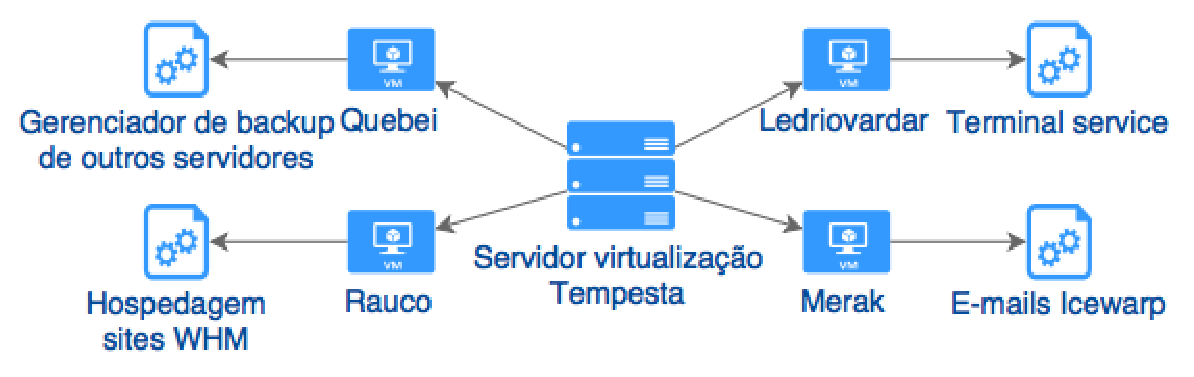
\includegraphics[width=350px]{img/servidor_tempesta.eps}
 }
 \caption{Servidor de virtualização Tempesta.}
 \label{fig:servidor_tempesta}
\end{figure}

\begin{itemize}
 \item \textit{Ledriovardar}: esse servidor possui 2 \textit{cores} para processamento, 2 GB de memória e 80 GB de disco. O servidor possui 
 o sistema operacional \textit{Windows 2008 Server R2} e possui o serviço de \textit{terminal service} para suporte e gerência de fibra 
 óptica do provedor;
 
 \item \textit{Merak}: esse servidor fornece serviço de \textit{e-mail}. Ele possui uma configuração de 6 \textit{cores} para processamento, 
 10 GB de memória e 1000 GB de disco. O servidor possui o sistema operacional \textit{Windows 2008 Server R2} e executa o \textit{software} 
 \textit{Icewarp Server 10.4.4} \cite{icewarp}. Essa aplicação fornece os serviços de envios de \textit{e-mails} (\ac{SMTP}), recebimentos 
 de \textit{e-mails} (\ac{POP} e \ac{IMAP}), Webmail (\ac{PHP}) e Anti-spam.
 Grande parte das contas estão ociosas pois são oferecidas juntamente com a internet vendida pelo provedor;
 %Possui ?? contas sendo que possui uma média de ?? usuários simultâneos...
 
 \item \textit{Quebei}: sua configuração é 1 \textit{core} de processamento, 3 GB de memória e 140 GB de disco. Esse servidor possui o 
 sistema operacional \textit{Ubuntu 14.04 \ac{LTS}} \cite{ubuntu} e sua função é gerenciar o \textit{backup} dos outros servidores. Para isso 
 ele utiliza a ferramenta \textit{Bacula 5.2.6} \cite{bacula} (pacote \textit{bacula-director-common 5.2.6}). Além disso, esse servidor possui 
 o sistema gerenciador de banco de dados \textit{MySQL 5.5.49} \cite{mysql} instalado, que esta configurado como \textit{master-slave}, sendo 
 que esse servidor é o \textit{slave} e o servidor \textit{Dati} (Seção \ref{section:servsemvirt}) é o \textit{master};
 
 \item \textit{Rauco}: esse servidor possui 2 \textit{cores} para processamento, 6 GB de memória e 600 GB de disco. Ele possui o sistema 
 operacional \textit{CentOS 6.8} \cite{centos}, sendo que esse servidor fornece o mesmo serviço do servidor \textit{Roncon} visto na 
 Seção \ref{section:serv_fulmine}), que é acesso a sites \textit{web} desenvolvidos com a linguagem \ac{PHP}.
\end{itemize}

\subsection{Servidor Tuono}
\label{section:serv_tuono}

O servidor Tuono possui quatro \ac{VM}s, como pode ser visto na Figura \ref{fig:servidor_tuono} juntamente com seus respectivos serviços. 
Esses serviços são listados a seguir:

\begin{figure}[h!]
 \centering
 \fcolorbox{black}{white}{
  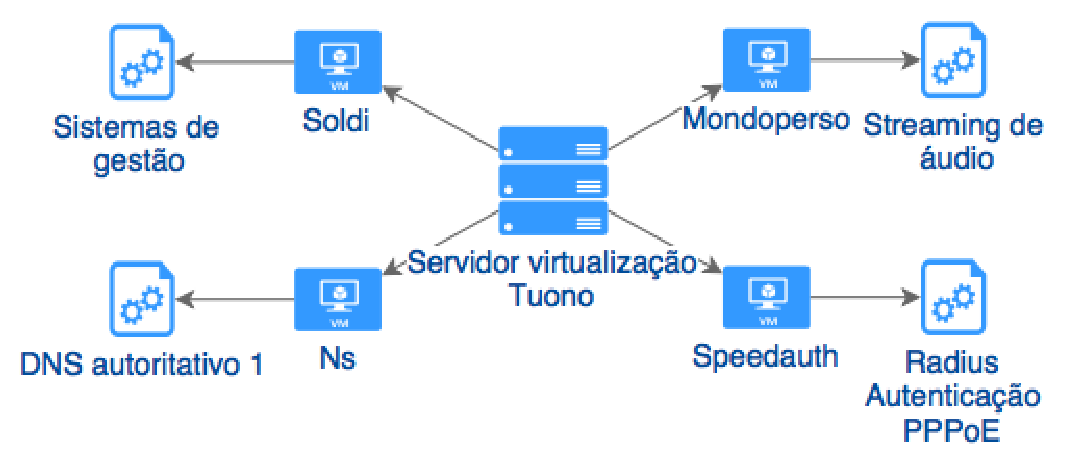
\includegraphics[width=300px]{img/servidor_tuono.eps}
 }
 \caption{Servidor de virtualização Tuono.}
 \label{fig:servidor_tuono}
\end{figure}

\begin{itemize}
 \item \textit{Mondoperso}: sua configuração é 1 \textit{core} de processamento, 512 MB de memória e 8 GB de disco. Esse servidor possui o 
 sistema operacional \textit{Ubuntu 14.04 \ac{LTS}} \cite{ubuntu} e fornece \textit{streaming} de áudio para web rádio, esse serviço é feito
 através do \textit{software} livre \textit{Icecast 2.3.3} \cite{icecast};
 
 \item \textit{Ns}: esse servidor possui 1 \textit{core} para processamento, 2 GB de memória e 30 GB de disco. O servidor possui o sistema 
 operacional \textit{CentOS 6.8} \cite{centos} e fornece, através do \textit{software} \textit{Bind 9.9.3} \cite{bind}, o serviço de \ac{DNS} 
 autoritativo e é o servidor de \ac{DNS} primário dos domínios hospedados pela empresa;

 \item \textit{Soldi}: sua configuração é 4 \textit{cores} de processamento, 4 GB de memória e 40 GB de disco. Esse servidor possui o 
 sistema operacional \textit{Ubuntu 14.04 \ac{LTS}} \cite{ubuntu} e é um servidor \textit{web} exclusivo para \textit{softwares} de gestão 
 desenvolvidos pela empresa. Os seguintes \textit{softwares} são utilizados: \textit{Apache 2.4.7} \cite{apache}, \textit{\ac{PHP} 5.5.9} \cite{php} 
 (com \textit{PHP-FPM 5.59}) e \textit{MySQL 5.5.49} \cite{mysql};

 \item \textit{Speedauth}: sua configuração é 2 \textit{cores} para processamento, 1,5 GB de memória e 8 GB de disco. O sistema operacional é o 
 \textit{Ubuntu 14.04 \ac{LTS}} \cite{ubuntu}, sendo que esse servidor fornece o mesmo serviço do servidor \textit{Masterauth} 
 (Seção \ref{section:serv_brina}), porém esse servidor possui a maior parte dos clientes.
\end{itemize}

\subsection{Servidor Venti}
\label{section:serv_venti}

O servidor Venti possui cinco \ac{VM}s, como pode ser visto na Figura \ref{fig:servidor_venti} juntamente com seus respectivos serviços. 
Esses serviços são listados a seguir:

\begin{figure}[h!]
 \centering
 \fcolorbox{black}{white}{
  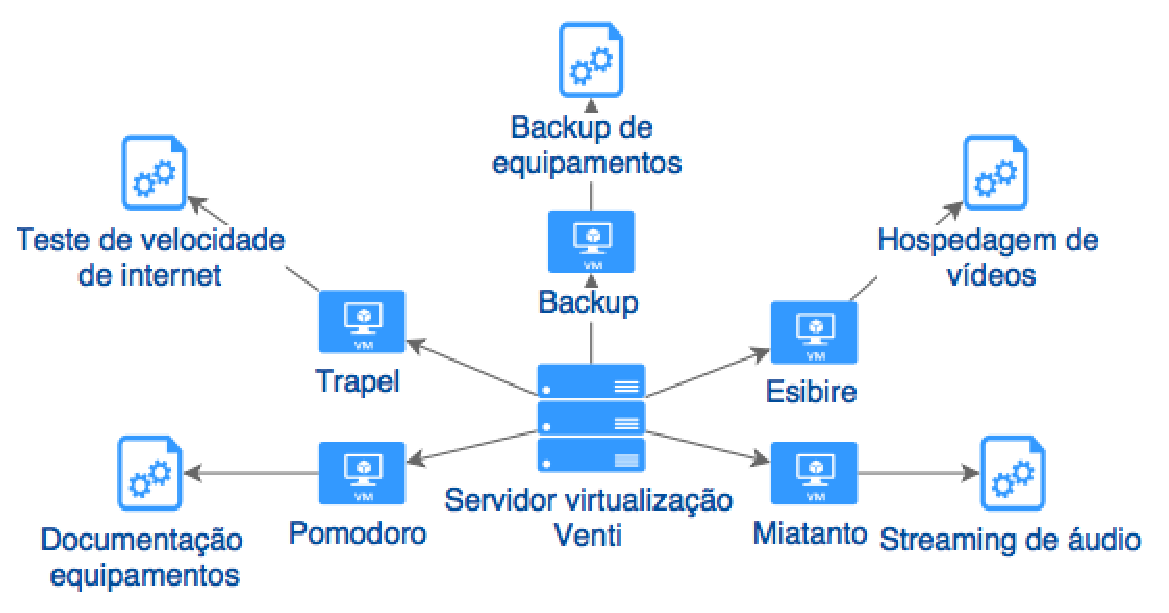
\includegraphics[width=340px]{img/servidor_venti.eps}
 }
 \caption{Servidor de virtualização Venti.}
 \label{fig:servidor_venti}
\end{figure}

\begin{itemize}
 \item \textit{Backup}: sua configuração é 1 \textit{core} para processamento, 1 GB de memória e 15 GB de disco. Esse servidor possui o 
 sistema operacional \textit{Ubuntu 14.04 \ac{LTS}} \cite{ubuntu} e executa o serviço de \textit{backup} dos equipamentos do provedor. Esse
 utiliza \textit{scripts} que foram desenvolvidos internamente e que buscam e copiam os dados através do protoccolo \ac{FTP};
 
 \item \textit{Esibire}: sua configuração é 1 \textit{core} para processamento, 1 GB de memória e 50 GB de disco. Esse servidor possui o 
 sistema operacional \textit{Ubuntu 14.04 \ac{LTS}} \cite{ubuntu} e faz a hospedagem de vídeos e a reprodução de \textit{streaming} utilizando
 \ac{FTP} e um servidor \textit{web} \textit{Apache 2.4.7};
 
 \item \textit{Miatanto}: sua configuração é 1 \textit{core} de processamento, 1 GB de memória e 8 GB de disco. Esse servidor possui o 
 sistema operacional \textit{Ubuntu 14.04 \ac{LTS}} \cite{ubuntu} e fornece \textit{streaming} de áudio para uma \textit{web} rádio, esse serviço 
 é feito através do \textit{software} livre \textit{Icecast 2.3.3} \cite{icecast};
 
 \item \textit{Pomodoro}: sua configuração é 1 \textit{core} de processamento, 2 GB de memória e 28 GB de disco. Esse servidor possui o 
 sistema operacional \textit{Ubuntu 14.04 \ac{LTS}} \cite{ubuntu} e armazena a documentação dos equipamentos do provedor, utilizando a aplicação
 de código aberto \textit{Sakai 2.9} \cite{sakai};
 
 \item \textit{Trapel}: sua configuração é 1 \textit{core} de processamento, 768 MB de memória e 8 GB de disco. Esse servidor possui o sistema 
 operacional \textit{Ubuntu 14.04 \ac{LTS}} \cite{ubuntu} e fornece um serviço de teste de velocidade da conexão de internet. Os usuários do 
 provedor utilizam esse serviço para testar a velocidade da sua internet. Para isso ele executa as aplicações \textit{Apache 2.4.7} \cite{apache} 
 e \textit{\ac{PHP} 5.5.9} \cite{php}, e um \textit{software} chamado \textit{SpeedTest} \cite{speedtest}.
\end{itemize}

%-graficos cpu memoria disco cada servidor de virtualizacao?? colocar aqui ou na implementacao??

\section{Considerações finais}

Neste capítulo foi apresentado a empresa e feito uma análise de seus serviços e definição dos serviços críticos. Com isso no próximo capítulo 
será desenvolvido uma proposta para implementação de um ambiente de alta disponibilidade nos servidores de virtualização da empresa, além de 
identificar as ferramentas que serão utilizadas para essa implementação.


%Esboço: \\
%-DNS (impacto direto para clientes e rede interna): \\
%requisicoes por segundo\\
%numero de usuarios\\
%-Radius (impacto direto para clientes): \\
%numero de usuarios autentidados em x tempo\\
%quantidade de dados armazenados no db em x tempo, tráfego utilizado, tempo conexao\\
%numero de usuarios\\
%-Sistemas (impacto indireto para clientes): \\
%gasto com funcionários ociosos\\
%quantidade de atendimento a clientes\\
%numero de cobrancas enviadas para clientes efetuar pagamento\\
%comunicacao entre setores e funcionários\\
%numero de usuarios\\
%-Telefonia (impacto indireto para clientes): \\
%quantidade de atendimento a clientes\\
%comunicacao entre setores e funcionários\\
%ligacoes saintes, atendimento, cobranca, tecnicos instalacoes internet\\
%numero de usuarios\\

